\documentclass[tikz,border=6mm]{standalone}
\usepackage{amsmath,amssymb}
\usepackage{fontspec}

\usetikzlibrary{positioning,arrows.meta,shapes.geometric,fit,backgrounds,calc}

% Define cohesive professional color palette
\definecolor{navyblue}{RGB}{30, 60, 105}
\definecolor{tealblue}{RGB}{20, 110, 105}
\definecolor{purplecat}{RGB}{95, 45, 120}
\definecolor{ambergold}{RGB}{180, 85, 15}
\definecolor{forestgreen}{RGB}{25, 115, 60}
\definecolor{crimsonred}{RGB}{175, 40, 40}
\definecolor{slategrey}{RGB}{70, 85, 100}

\begin{document}
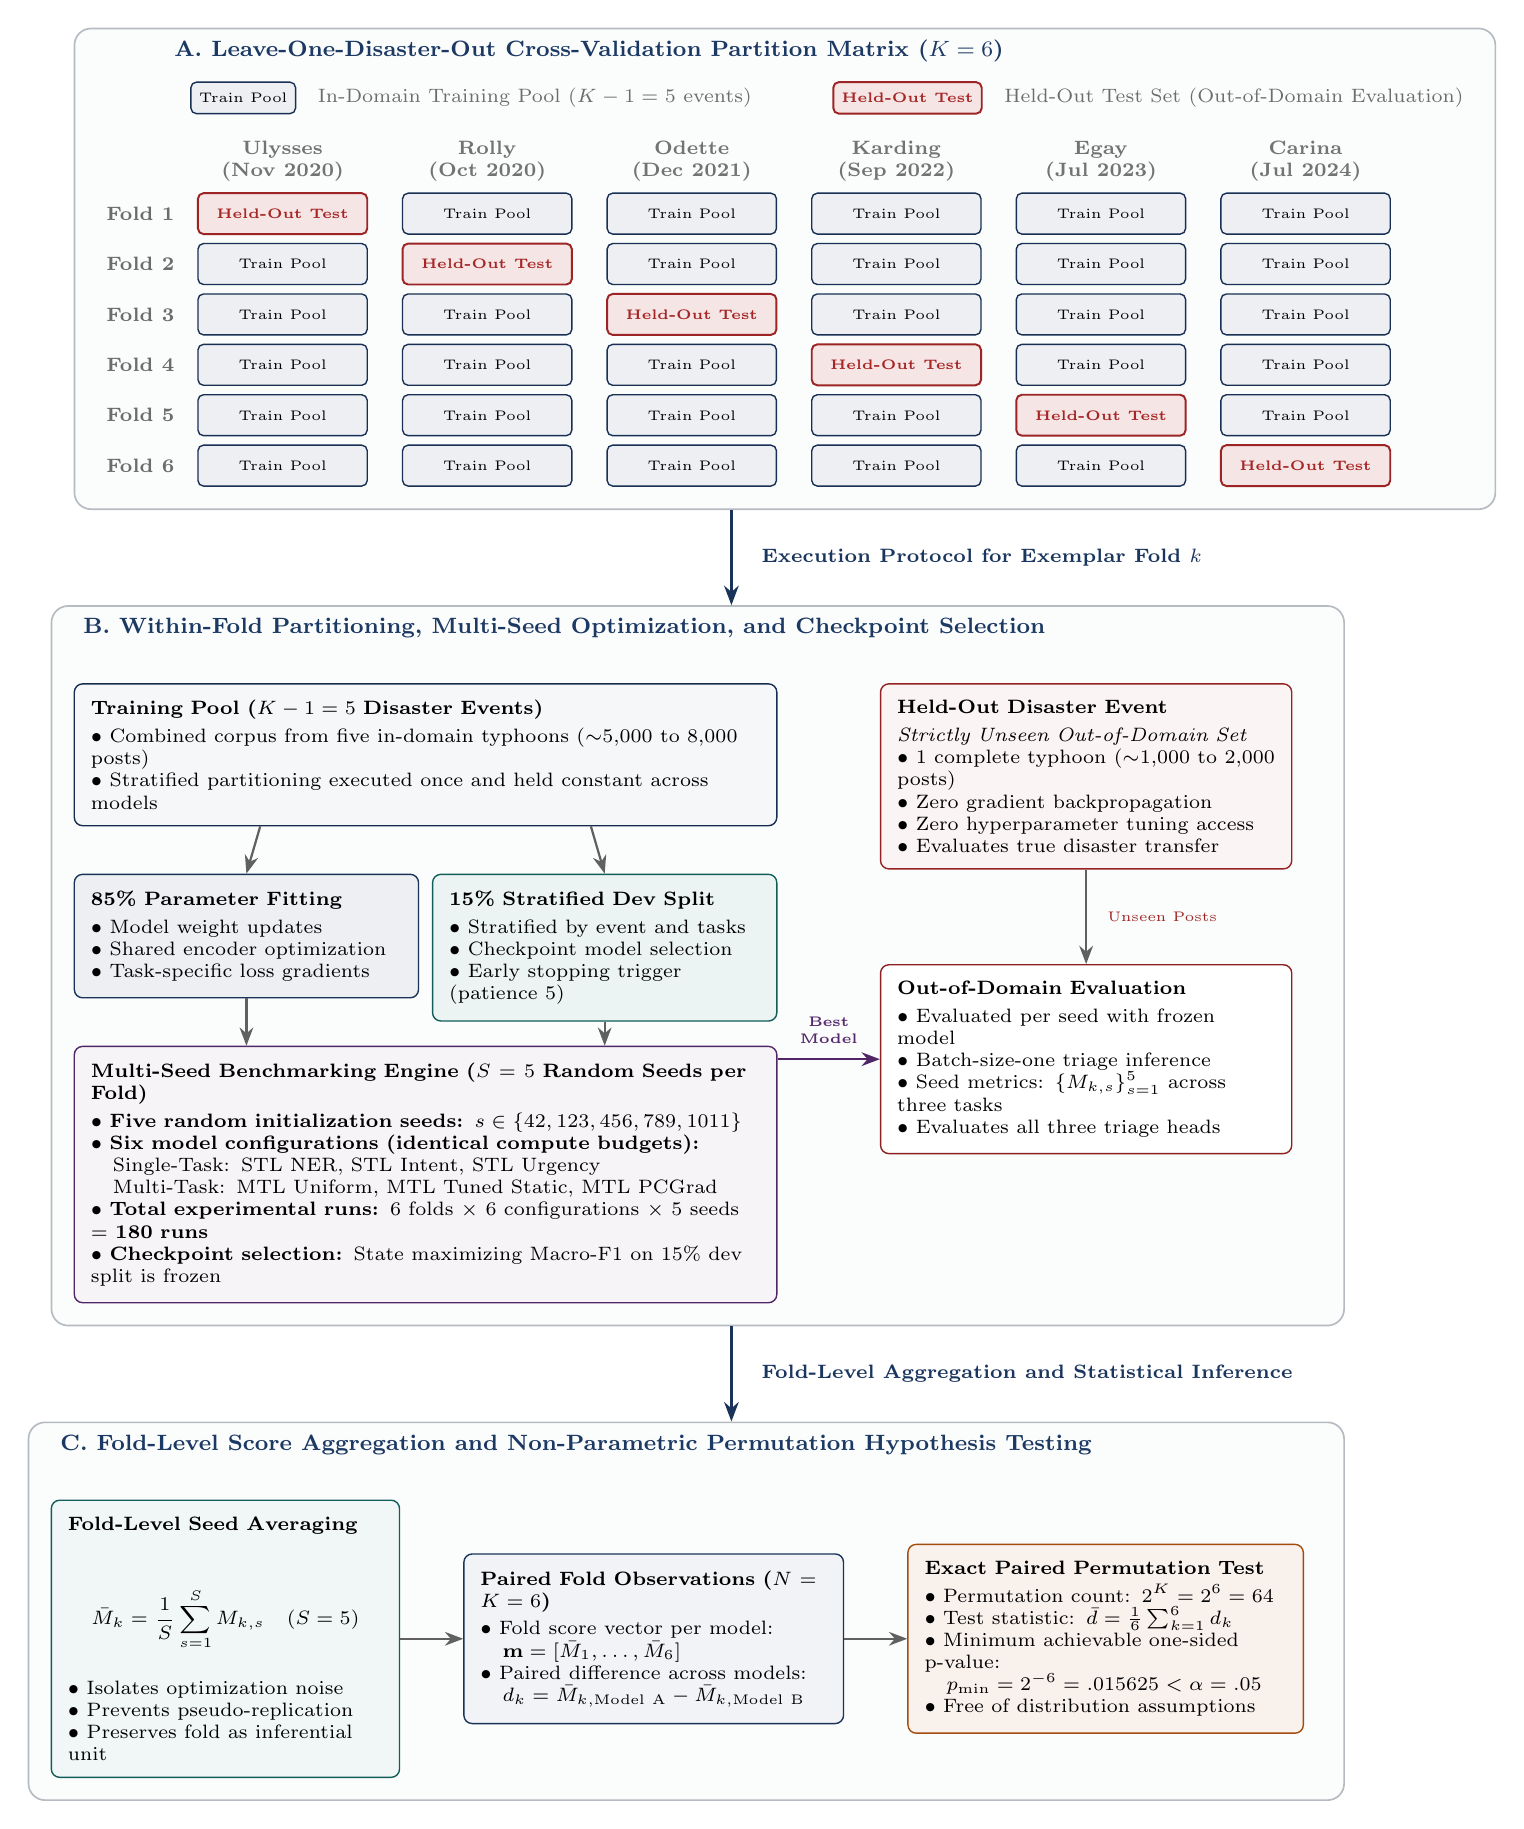
\begin{tikzpicture}[
    font=\small,
    >=Stealth,
    every node/.append style={execute at begin node={\hyphenpenalty=10000\exhyphenpenalty=10000\relax}},
    % Styles
    sectiontitle/.style={
        font=\bfseries\footnotesize,
        text=navyblue!95!black,
        anchor=west
    },
    colheader/.style={
        font=\bfseries\scriptsize,
        text=gray!90!black,
        align=center
    },
    foldlbl/.style={
        font=\bfseries\scriptsize,
        text=gray!85!black,
        align=right,
        anchor=east
    },
    celltrain/.style={
        draw=navyblue!80!black,
        fill=navyblue!8,
        rounded corners=2pt,
        align=center,
        inner sep=3pt,
        font=\tiny,
        line width=0.5pt,
        minimum width=2.15cm,
        minimum height=0.52cm
    },
    celltest/.style={
        draw=crimsonred!90!black,
        fill=crimsonred!12,
        rounded corners=2pt,
        align=center,
        inner sep=3pt,
        font=\tiny\bfseries,
        text=crimsonred!95!black,
        line width=0.7pt,
        minimum width=2.15cm,
        minimum height=0.52cm
    },
    subcard/.style={
        draw=gray!50,
        fill=white,
        rounded corners=3pt,
        align=left,
        inner sep=6pt,
        font=\scriptsize,
        line width=0.5pt
    },
    flowarrow/.style={
        ->,
        thick,
        draw=gray!75!black
    },
    accentarrow/.style={
        ->,
        thick,
        draw=purplecat!85!black
    }
]

    % Global Canvas Boundary Anchors to guarantee perfect vertical alignment across all 3 panels
    \coordinate (canvas_left) at (-0.3, 0);
    \coordinate (canvas_right) at (14.7, 0);

    % =========================================================================
    % PANEL A: LODO CROSS-VALIDATION MATRIX (6 FOLDS X 6 DISASTERS)
    % =========================================================================
    \node[sectiontitle] (titleA) at (0.0, 0.85) {A. Leave-One-Disaster-Out Cross-Validation Partition Matrix ($K = 6$)};

    % Clean Dedicated Legend Row below Title
    \node[celltrain, minimum width=1.3cm, minimum height=0.4cm] (leg_train) at (1.0, 0.25) {Train Pool};
    \node[font=\scriptsize, right=0.15cm of leg_train, text=gray!85!black] (leg_train_lbl) {In-Domain Training Pool ($K-1=5$ events)};
    \node[celltest, minimum width=1.4cm, minimum height=0.4cm, right=0.9cm of leg_train_lbl] (leg_test) {Held-Out Test};
    \node[font=\scriptsize, right=0.15cm of leg_test, text=gray!85!black] (leg_test_lbl) {Held-Out Test Set (Out-of-Domain Evaluation)};

    % Grid Column Headers (6 Disasters)
    \node[colheader, text width=2.15cm] (h1) at (1.5, -0.55) {\textbf{Ulysses}\\(Nov 2020)};
    \node[colheader, text width=2.15cm, right=0.2cm of h1] (h2) {\textbf{Rolly}\\(Oct 2020)};
    \node[colheader, text width=2.15cm, right=0.2cm of h2] (h3) {\textbf{Odette}\\(Dec 2021)};
    \node[colheader, text width=2.15cm, right=0.2cm of h3] (h4) {\textbf{Karding}\\(Sep 2022)};
    \node[colheader, text width=2.15cm, right=0.2cm of h4] (h5) {\textbf{Egay}\\(Jul 2023)};
    \node[colheader, text width=2.15cm, right=0.2cm of h5] (h6) {\textbf{Carina}\\(Jul 2024)};

    % Folds Rows (Folds 1 to 6) with clean vertical step
    % Fold 1 (Holdout: Ulysses)
    \node[foldlbl] (f1lbl) at (0.25, -1.22) {Fold 1};
    \node[celltest] (f1c1) at (h1 |- f1lbl) {Held-Out Test};
    \node[celltrain] (f1c2) at (h2 |- f1lbl) {Train Pool};
    \node[celltrain] (f1c3) at (h3 |- f1lbl) {Train Pool};
    \node[celltrain] (f1c4) at (h4 |- f1lbl) {Train Pool};
    \node[celltrain] (f1c5) at (h5 |- f1lbl) {Train Pool};
    \node[celltrain] (f1c6) at (h6 |- f1lbl) {Train Pool};

    % Fold 2 (Holdout: Rolly)
    \node[foldlbl] (f2lbl) at (0.25, -1.86) {Fold 2};
    \node[celltrain] (f2c1) at (h1 |- f2lbl) {Train Pool};
    \node[celltest] (f2c2) at (h2 |- f2lbl) {Held-Out Test};
    \node[celltrain] (f2c3) at (h3 |- f2lbl) {Train Pool};
    \node[celltrain] (f2c4) at (h4 |- f2lbl) {Train Pool};
    \node[celltrain] (f2c5) at (h5 |- f2lbl) {Train Pool};
    \node[celltrain] (f2c6) at (h6 |- f2lbl) {Train Pool};

    % Fold 3 (Holdout: Odette)
    \node[foldlbl] (f3lbl) at (0.25, -2.50) {Fold 3};
    \node[celltrain] (f3c1) at (h1 |- f3lbl) {Train Pool};
    \node[celltrain] (f3c2) at (h2 |- f3lbl) {Train Pool};
    \node[celltest] (f3c3) at (h3 |- f3lbl) {Held-Out Test};
    \node[celltrain] (f3c4) at (h4 |- f3lbl) {Train Pool};
    \node[celltrain] (f3c5) at (h5 |- f3lbl) {Train Pool};
    \node[celltrain] (f3c6) at (h6 |- f3lbl) {Train Pool};

    % Fold 4 (Holdout: Karding)
    \node[foldlbl] (f4lbl) at (0.25, -3.14) {Fold 4};
    \node[celltrain] (f4c1) at (h1 |- f4lbl) {Train Pool};
    \node[celltrain] (f4c2) at (h2 |- f4lbl) {Train Pool};
    \node[celltrain] (f4c3) at (h3 |- f4lbl) {Train Pool};
    \node[celltest] (f4c4) at (h4 |- f4lbl) {Held-Out Test};
    \node[celltrain] (f4c5) at (h5 |- f4lbl) {Train Pool};
    \node[celltrain] (f4c6) at (h6 |- f4lbl) {Train Pool};

    % Fold 5 (Holdout: Egay)
    \node[foldlbl] (f5lbl) at (0.25, -3.78) {Fold 5};
    \node[celltrain] (f5c1) at (h1 |- f5lbl) {Train Pool};
    \node[celltrain] (f5c2) at (h2 |- f5lbl) {Train Pool};
    \node[celltrain] (f5c3) at (h3 |- f5lbl) {Train Pool};
    \node[celltrain] (f5c4) at (h4 |- f5lbl) {Train Pool};
    \node[celltest] (f5c5) at (h5 |- f5lbl) {Held-Out Test};
    \node[celltrain] (f5c6) at (h6 |- f5lbl) {Train Pool};

    % Fold 6 (Holdout: Carina)
    \node[foldlbl] (f6lbl) at (0.25, -4.42) {Fold 6};
    \node[celltrain] (f6c1) at (h1 |- f6lbl) {Train Pool};
    \node[celltrain] (f6c2) at (h2 |- f6lbl) {Train Pool};
    \node[celltrain] (f6c3) at (h3 |- f6lbl) {Train Pool};
    \node[celltrain] (f6c4) at (h4 |- f6lbl) {Train Pool};
    \node[celltrain] (f6c5) at (h5 |- f6lbl) {Train Pool};
    \node[celltest] (f6c6) at (h6 |- f6lbl) {Held-Out Test};

    % Background Box for Panel A
    \begin{scope}[on background layer]
        \node[draw=slategrey!40, fill=slategrey!2, rounded corners=6pt, line width=0.6pt,
              fit=(canvas_left |- titleA)(canvas_right |- titleA)(f1lbl)(f6lbl)(h6)(f6c6)(leg_test_lbl), inner sep=8pt] (boxA) {};
    \end{scope}

    % =========================================================================
    % PANEL B: WITHIN-FOLD PARTITIONING & MULTI-SEED EXPERIMENTAL RUNS
    % Generous 1.5cm vertical clearance below Box A
    % =========================================================================
    \node[sectiontitle, below=1.5cm of boxA.south west, anchor=west] (titleB) 
        {B. Within-Fold Partitioning, Multi-Seed Optimization, and Checkpoint Selection};

    % Left Container: Training Pool Pipeline
    \node[subcard, below=0.45cm of titleB.south west, anchor=north west, draw=navyblue!75!black, fill=navyblue!4, text width=8.5cm] (pool_box) {
        \textbf{Training Pool ($K-1 = 5$ Disaster Events)}\\[2pt]
        $\bullet$ Combined corpus from five in-domain typhoons ($\sim$5,000 to 8,000 posts)\\
        $\bullet$ Stratified partitioning executed once and held constant across models
    };

    % Train Split & Dev Split
    \node[subcard, below=0.6cm of pool_box.south west, anchor=north west, draw=navyblue!85!black, fill=navyblue!8, text width=3.95cm] (train_split) {
        \textbf{85\% Parameter Fitting}\\[2pt]
        $\bullet$ Model weight updates\\
        $\bullet$ Shared encoder optimization\\
        $\bullet$ Task-specific loss gradients
    };

    \node[subcard, below=0.6cm of pool_box.south east, anchor=north east, draw=tealblue!85!black, fill=tealblue!8, text width=3.95cm] (dev_split) {
        \textbf{15\% Stratified Dev Split}\\[2pt]
        $\bullet$ Stratified by event and tasks\\
        $\bullet$ Checkpoint model selection\\
        $\bullet$ Early stopping trigger (patience 5)
    };

    \draw[flowarrow] ($(pool_box.south) + (-2.1, 0)$) -- (train_split.north);
    \draw[flowarrow] ($(pool_box.south) + (2.1, 0)$) -- (dev_split.north);

    % Training Engine Card
    \node[subcard, below=0.6cm of train_split.south west, anchor=north west, draw=purplecat!85!black, fill=purplecat!5, text width=8.5cm] (engine_box) {
        \textbf{Multi-Seed Benchmarking Engine ($S = 5$ Random Seeds per Fold)}\\[2pt]
        $\bullet$ \textbf{Five random initialization seeds:} $s \in \{42, 123, 456, 789, 1011\}$\\
        $\bullet$ \textbf{Six model configurations (identical compute budgets):}\\
        \quad Single-Task: STL NER, STL Intent, STL Urgency\\
        \quad Multi-Task: MTL Uniform, MTL Tuned Static, MTL PCGrad\\
        $\bullet$ \textbf{Total experimental runs:} 6 folds $\times$ 6 configurations $\times$ 5 seeds = \textbf{180 runs}\\
        $\bullet$ \textbf{Checkpoint selection:} State maximizing Macro-F1 on 15\% dev split is frozen
    };

    \draw[flowarrow] (train_split.south) -- (train_split.south |- engine_box.north);
    \draw[flowarrow] (dev_split.south) -- (dev_split.south |- engine_box.north);

    % Right Container: Out-of-Domain Held-Out Evaluation (1.3cm Gap)
    \node[subcard, right=1.3cm of pool_box.north east, anchor=north west, draw=crimsonred!85!black, fill=crimsonred!5, text width=4.8cm] (ood_box) {
        \textbf{Held-Out Disaster Event}\\[2pt]
        \textit{Strictly Unseen Out-of-Domain Set}\\
        $\bullet$ 1 complete typhoon ($\sim$1,000 to 2,000 posts)\\
        $\bullet$ Zero gradient backpropagation\\
        $\bullet$ Zero hyperparameter tuning access\\
        $\bullet$ Evaluates true disaster transfer
    };

    % Inference Evaluation Card
    \node[subcard, below=1.2cm of ood_box, draw=crimsonred!80!black, fill=white, text width=4.8cm] (eval_box) {
        \textbf{Out-of-Domain Evaluation}\\[2pt]
        $\bullet$ Evaluated per seed with frozen model\\
        $\bullet$ Batch-size-one triage inference\\
        $\bullet$ Seed metrics: $\{M_{k, s}\}_{s=1}^5$ across three tasks\\
        $\bullet$ Evaluates all three triage heads
    };

    \draw[flowarrow] (ood_box.south) -- node[midway, right=4pt, font=\tiny, text=crimsonred!90!black] {Unseen Posts} (eval_box.north);
    \draw[accentarrow] (engine_box.east |- eval_box.west) -- node[midway, above=2pt, font=\tiny\bfseries, align=center, text=purplecat!90!black] {Best\\Model} (eval_box.west);

    % Background Box for Panel B
    \begin{scope}[on background layer]
        \node[draw=slategrey!40, fill=slategrey!2, rounded corners=6pt, line width=0.6pt,
              fit=(canvas_left |- titleB)(canvas_right |- titleB)(pool_box)(train_split)(engine_box)(ood_box)(eval_box), inner sep=8pt] (boxB) {};
    \end{scope}

    % =========================================================================
    % PANEL C: FOLD AGGREGATION & SIGN-FLIP PERMUTATION TESTING
    % Generous 1.5cm vertical clearance below Box B
    % =========================================================================
    \node[sectiontitle, below=1.5cm of boxB.south west, anchor=west] (titleC) 
        {C. Fold-Level Score Aggregation and Non-Parametric Permutation Hypothesis Testing};

    % Step 1: Seed Averaging
    \node[subcard, below=0.45cm of titleC.south west, anchor=north west, draw=tealblue!85!black, fill=tealblue!6, text width=4.0cm] (agg_box) {
        \textbf{Fold-Level Seed Averaging}\\[2pt]
        $$\bar{M}_k = \frac{1}{S} \sum_{s=1}^{S} M_{k, s} \quad (S = 5)$$
        $\bullet$ Isolates optimization noise\\
        $\bullet$ Prevents pseudo-replication\\
        $\bullet$ Preserves fold as inferential unit
    };

    % Step 2: N=6 Paired Observations (Generous 0.8cm Gap)
    \node[subcard, right=0.8cm of agg_box, draw=navyblue!85!black, fill=navyblue!6, text width=4.4cm] (obs_box) {
        \textbf{Paired Fold Observations ($N = K = 6$)}\\[2pt]
        $\bullet$ Fold score vector per model:\\
        \quad $\mathbf{m} = [\bar{M}_1, \dots, \bar{M}_6]$\\
        $\bullet$ Paired difference across models:\\
        \quad $d_k = \bar{M}_{k, \text{Model A}} - \bar{M}_{k, \text{Model B}}$
    };

    % Step 3: Exact Permutation Test (Generous 0.8cm Gap)
    \node[subcard, right=0.8cm of obs_box, draw=ambergold!90!black, fill=ambergold!8, text width=4.6cm] (perm_box) {
        \textbf{Exact Paired Permutation Test}\\[2pt]
        $\bullet$ Permutation count: $2^K = 2^6 = 64$\\
        $\bullet$ Test statistic: $\bar{d} = \frac{1}{6}\sum_{k=1}^6 d_k$\\
        $\bullet$ Minimum achievable one-sided p-value:\\
        \quad $p_{\min} = 2^{-6} = .015625 < \alpha = .05$\\
        $\bullet$ Free of distribution assumptions
    };

    \draw[flowarrow] (agg_box.east) -- (obs_box.west);
    \draw[flowarrow] (obs_box.east) -- (perm_box.west);

    % Background Box for Panel C
    \begin{scope}[on background layer]
        \node[draw=slategrey!40, fill=slategrey!2, rounded corners=6pt, line width=0.6pt,
              fit=(canvas_left |- titleC)(canvas_right |- titleC)(agg_box)(obs_box)(perm_box), inner sep=8pt] (boxC) {};
    \end{scope}

    % =========================================================================
    % MAJOR INTER-PANEL TRANSITION ARROWS
    % Strictly vertical, centered plumb-lines connecting container boundaries
    % =========================================================================
    \coordinate (center_x) at (7.2, 0);

    \draw[flowarrow, line width=0.9pt, draw=navyblue!85!black] (center_x |- boxA.south) -- (center_x |- boxB.north)
        node[midway, right=0.25cm, font=\scriptsize\bfseries, text=navyblue!90!black] {Execution Protocol for Exemplar Fold $k$};

    \draw[flowarrow, line width=0.9pt, draw=navyblue!85!black] (center_x |- boxB.south) -- (center_x |- boxC.north)
        node[midway, right=0.25cm, font=\scriptsize\bfseries, text=navyblue!90!black] {Fold-Level Aggregation and Statistical Inference};

\end{tikzpicture}
\end{document}
